\scanpage{125}
% archive sheet number: 124
% source lines 1--11
semisimple, \rlap{,}we have a category which is no longer graded, only filtered, \deleted{I} If $V$ is the category of schemes of finite type over a fixed field, $M$ the category of motives over this same field (\rlap{a}p\rlap{v}resumed with all the data and conditions of 1º\rlap{)}\handwritten{)}\handwritten{\unsure{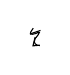
\begin{tikzpicture}[x=.4cm,y=.4cm,baseline=-.2ex]\draw (.12,.45) .. controls (-.04,.23) and (.01,.24) .. (.20,.28) .. controls (.34,.36) and (.36,.34) .. (.18,.12) .. controls (.10,-.03) and (.21,-.10) .. (.33,-.10);\draw (.02,.27)--(.35,.38);\draw (.18,.17)--(.11,-.11)--(.32,-.09);\end{tikzpicture}|\deleted{(}}}, we must have a functor \deleted{\unsure{$V$|$Y$}} compatible with these structures \deleted{of} (motivic cohomology)
\[
h:V\handwritten{\longrightarrow}\unsure{\rlap{\(\mathrm E\)}G|\mathbb{G}|G|E}\mathrm{rad}(M)\handwritten{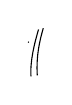
\begin{tikzpicture}[x=.4cm,y=.4cm,baseline=-.2ex]\draw (.08,-.75) .. controls (.04,-.20) and (.25,.50) .. (.32,.74);\draw (.28,-.72) .. controls (.24,-.10) and (.36,.40) .. (.47,.78);\fill (0,.34) circle (.025);\end{tikzpicture}}\quad\text{(Koko structure on }\mathrm{Grad}(M)\text{)}\handwritten{,}
\]
and we desire that the usual cohomological functors on $V$ factor\unsure{i\rlap{n}ng|i\rlap{r}ng|i\rlap{e}ng} through \deleted{$M$. This imposes}\inserted{functors on $M$. We shall want\handwritten{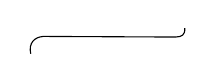
\begin{tikzpicture}[x=.4cm,y=.4cm,baseline=-.2ex]\draw (0,-.35) .. controls (-.08,.0) and (.13,.18) .. (.40,.20)--(4.6,.18) .. controls (4.80,.19) and (4.90,.24) .. (4.89,.46);\end{tikzpicture}}} that the \deleted{fibre} functors obtained on $M$ b\rlap{n}\unsure{\rlap{e}\rlap{t}e|\rlap{t}e}\rlap{t} \deleted{only \uline{twisted}} genuine fibre functors\inserted{\handwritten{(not twisted)}\handwritten{\begin{tikzpicture}[x=.4cm,y=.4cm,baseline=-.2ex]\draw (0,-.40) .. controls (.18,-.12) and (.28,.02) .. (.54,.07)--(2.70,.38) .. controls (2.86,.40) and (2.99,.45) .. (2.96,.63);\end{tikzpicture}}}, which is not silly, \deleted{for}\inserted{\handwritten{\unsure{For|for}}} we had put the Koko symmetry structure on $\mathrm{Grad}(M)$: we have thus got rid once and for all of the ``twisting''.

% source lines 12--15
We can also, to speak of genuine fibre functors on the category of semisimple motives, replace the ``geometric'' symmetry datum i.e. Koko's for the tensor product in \deleted{$\mathrm{Grad}(M)$}\inserted{the graded category $M$\handwritten{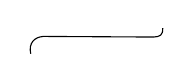
\begin{tikzpicture}[x=.4cm,y=.4cm,baseline=-.2ex]\draw (0,-.35) .. controls (-.08,.0) and (.13,.18) .. (.40,.20)--(3.9,.18) .. controls (4.10,.19) and (4.20,.24) .. (4.19,.46);\end{tikzpicture}}}, by the same one doctored by the sign $(-1)^{ij}$ when we have \unsure{\rlap{r}a\rlap{a}r|$\mathbb{a}\mathbb{r}$}guments of degree $i,j$.

% source lines 16--24
11) Of course, it is appropriate to seek intrinsic structure theorems, in terms of gerbes, for categories $\unsure{\rlap{\(\mathrm N\)}C|\handwritten{\mathfrak{C}}|\handwritten{\mathscr{C}}|\mathbb{C}}$ equipped with the structures of 1º,\inserted{with $k=\mathrm{End}(\underline{1})$ a given field.\handwritten{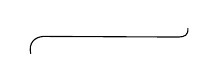
\begin{tikzpicture}[x=.4cm,y=.4cm,baseline=-.2ex]\draw (0,-.35) .. controls (-.08,.0) and (.13,.18) .. (.40,.20)--(4.7,.18) .. controls (4.90,.19) and (5.00,.24) .. (4.99,.46);\end{tikzpicture}}} It is appropriate if need be to assume that there exists an extension of $k$ over which there is a graded t\rlap{r}w\rlap{o}isted fibre functor (or m\unsure{\rlap{u}ul|\rlap{b}ul|ul}tigraded ? But where to stop ? ). The finest would obviously be to find a g\rlap{g}eneral structure theorem, without \uline{assuming} the existence of a more or less twisted fibre functor anywhere at all, by defining a sufficiently general notion of twisted fibre functor (?) and by \unsure{\rlap{r}p|p|$\mathbb{p}$}\rlap{r}r\unsure{\rlap{u}o|o}v\rlap{q}ing that th\rlap{p}ere are always some over a suitable extension of $k$.
